\documentclass{beamer}
%
% Choose how your presentation looks.
%
% For more themes, color themes and font themes, see:
% http://deic.uab.es/~iblanes/beamer_gallery/index_by_theme.html
%
\mode<presentation>
{
  \usetheme{default}      % or try Darmstadt, Madrid, Warsaw, ...
  \usecolortheme{default} % or try albatross, beaver, crane, ...
  \usefonttheme{default}  % or try serif, structurebold, ...
  \setbeamertemplate{navigation symbols}{}
  \setbeamertemplate{caption}[numbered]
} 

\usepackage[english]{babel}
\usepackage[utf8x]{inputenc}
\usepackage{comment}

\setbeamerfont{page number in head/foot}{size=\scriptsize}
\setbeamertemplate{footline}[frame number]
\let\otp\titlepage
\renewcommand{\titlepage}{\otp\addtocounter{framenumber}{-1}}

\title{Deep Learning application \\ to large-scale image retrieval }
\author{Pavel Nesterov}
\institute{\url{http://pavelnesterov.info/}}
\date{\today}

\begin{document}

\begin{frame}[plain]
  \titlepage
\end{frame}


% Uncomment these lines for an automatically generated outline.
%\begin{frame}{Outline}
%  \tableofcontents
%\end{frame}

\section{Introduction}


\begin{frame}{Classical approach}

\begin{figure}[h!]
  \centering
  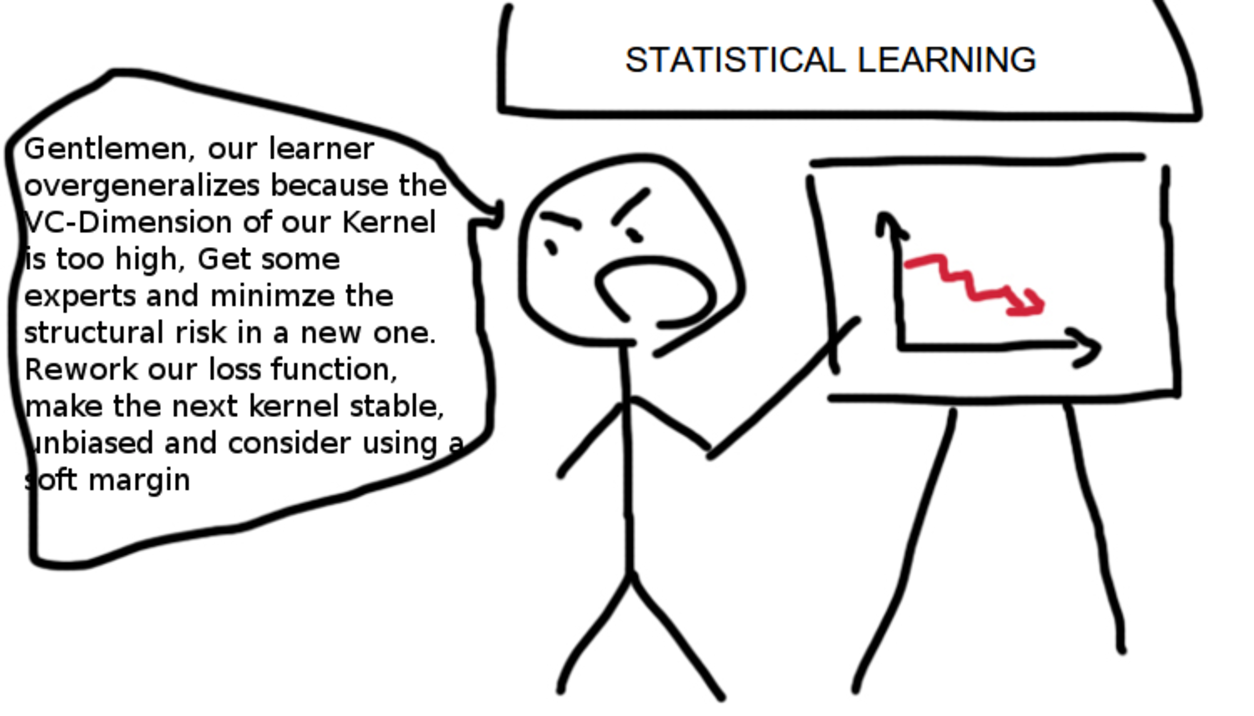
\includegraphics[width=1\textwidth]{images/stat.png}
\end{figure}

\end{frame}


\begin{frame}{Modern approach}

\begin{figure}[h!]
  \centering
  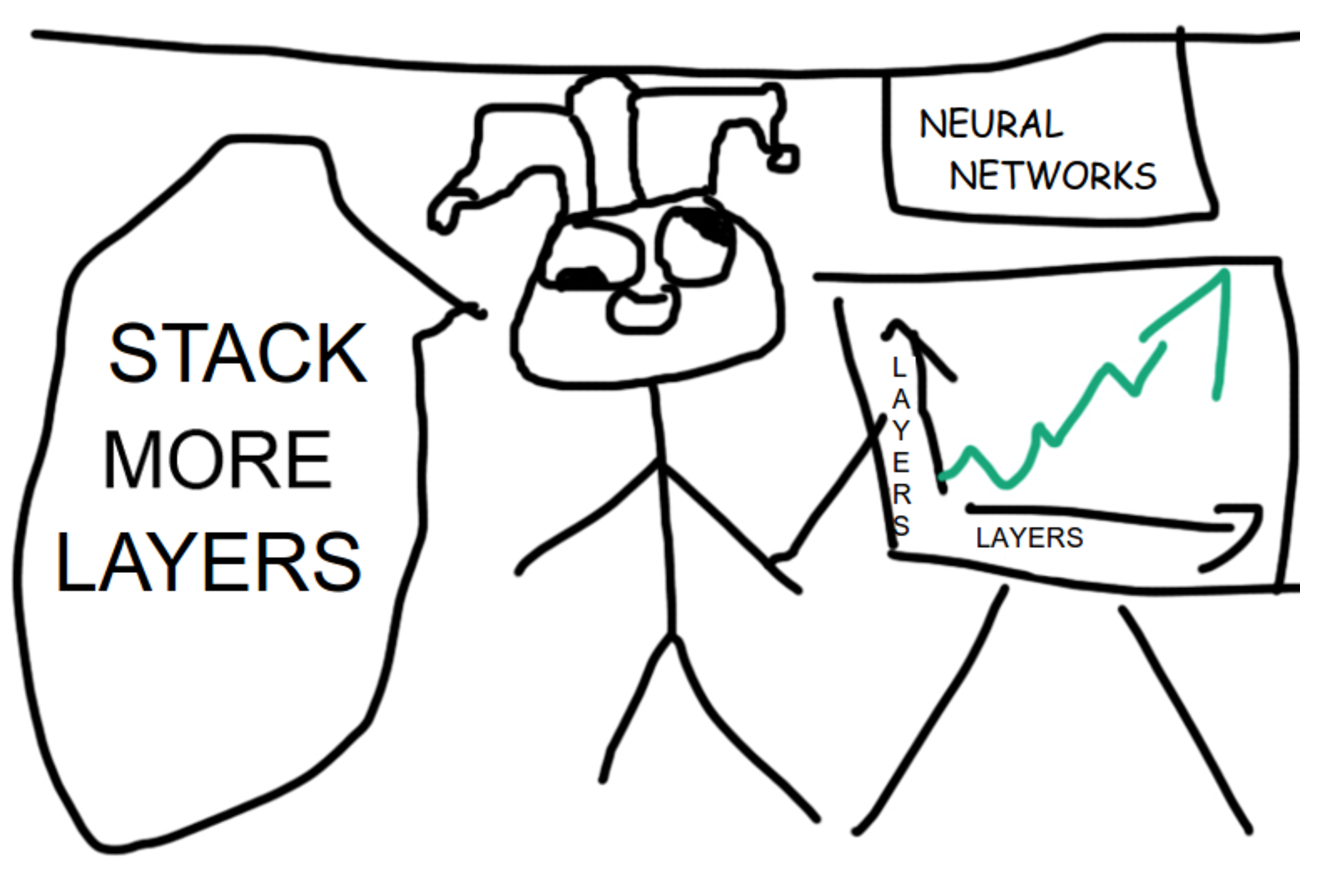
\includegraphics[width=1\textwidth]{images/nn.png}
\end{figure}

\end{frame}


\begin{frame}{Linear models}

\begin{columns}[t]
\column{0.5\textwidth}

\begin{block}{Linear regression}
\begin{eqnarray*}
\hat{y} &=& w_0 + \sum_{i=1}^N w_i x_i
\end{eqnarray*}
\end{block}	
	
\column{0.5\textwidth}

\begin{block}{Logistic regression}

\begin{eqnarray*}
\hat{p}\left(y = 1\right) &=& \sigma\left(w_0 + \sum_{i=1}^N w_i x_i\right) \\
\sigma\left(x\right) &=& \frac{1}{1 + e^{-x}}
\end{eqnarray*}
\end{block}
	
\end{columns}

\end{frame}


\begin{frame}{Biological neuron}

\begin{figure}[h!]
  \centering
  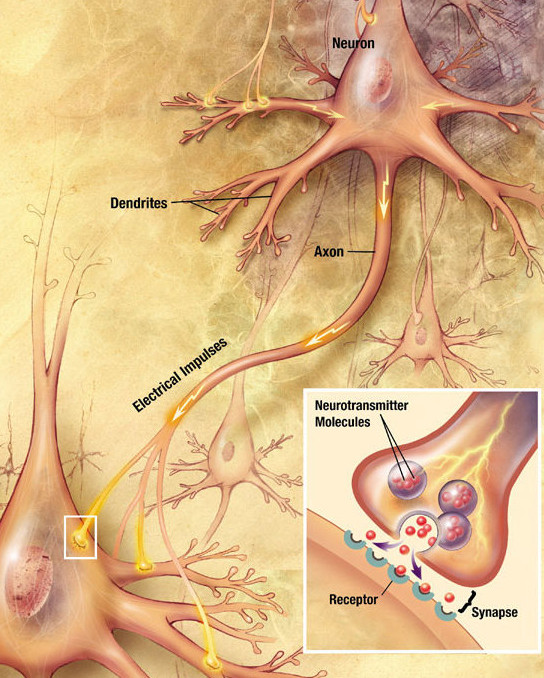
\includegraphics[width=0.6\textwidth]{images/bneuron.jpg}
\end{figure}

\end{frame}


\begin{frame}{Artificial neuron}

\begin{figure}[h!]
  \centering
  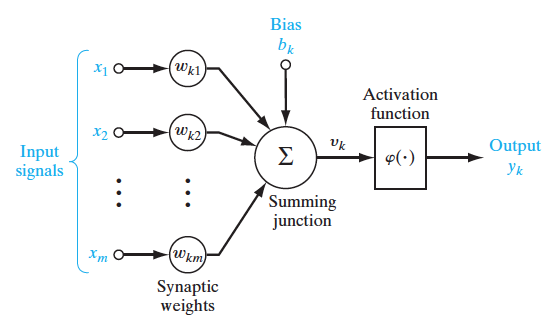
\includegraphics[width=1\textwidth]{images/aneuron.png}
\end{figure}

\begin{itemize}
\item 
\end{itemize}

\end{frame}


\begin{frame}{Single layer network}

\begin{columns}[t]
\column{0.5\textwidth}

\begin{figure}[h!]
  \centering
  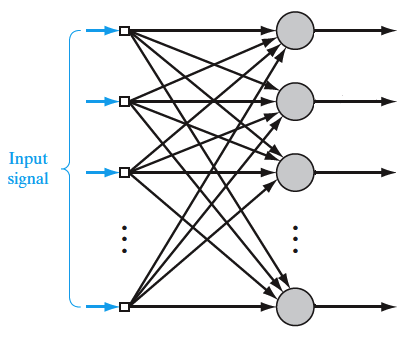
\includegraphics[width=1\textwidth]{images/single_layer.png}
\end{figure}	

\column{0.5\textwidth}

\begin{block}{MaxEnt model}
\begin{eqnarray*}
\hat{h}_k &=& w_{k, 0} + \sum_{i=1}^N w_{k, i} x_i \\
\hat{p}\left(y = C_k\right) &=& \frac{e^{h_k}}{\sum_{j=1}^K e^{h_j}}
\end{eqnarray*}
\end{block}
	
\end{columns}

\end{frame}


\begin{frame}{Shallow network}

\begin{figure}[h!]
  \centering
  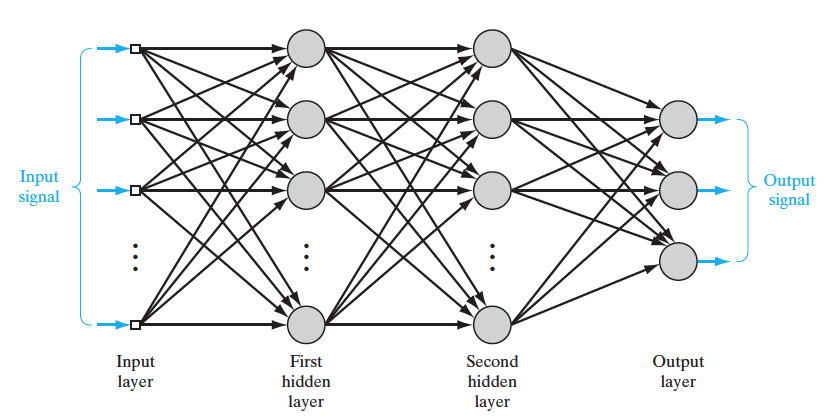
\includegraphics[width=1\textwidth]{images/mlp.png}
\end{figure}

\begin{itemize}
\item \textit{how many parameters second hidden layer requires?}
\end{itemize}

\end{frame}


\begin{frame}{What next?}

\begin{figure}[h!]
  \centering
  
\includegraphics[width=1\textwidth]{images/inception.png}
\end{figure}

\begin{itemize}
\item solution is to simplify network
\end{itemize}

\end{frame}


\begin{frame}{Convolutions}

\begin{figure}[h!]
  \centering
  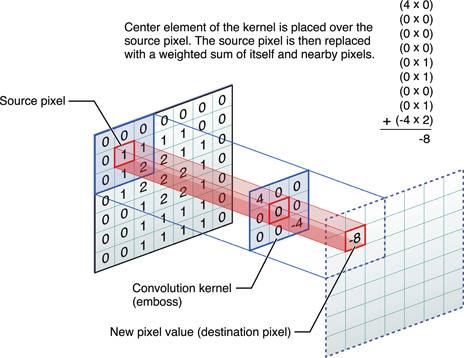
\includegraphics[width=1\textwidth]{images/kernel_convolution.jpg}
\end{figure}

\end{frame}


\begin{frame}{Filter bank}

\begin{figure}[h!]
  \centering
  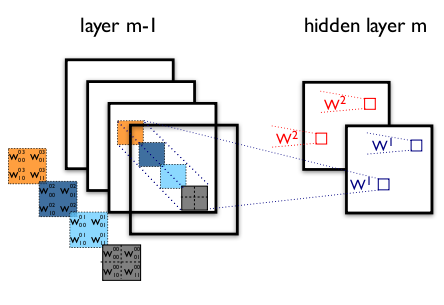
\includegraphics[width=1\textwidth]{images/cnn_explained.png}
\end{figure}

\begin{itemize}
\item \textit{how many parameters second convolutional hidden layer requires now?}
\end{itemize}

\end{frame}


\begin{frame}{Deep convolutional network}

\begin{figure}[h!]
  \centering
  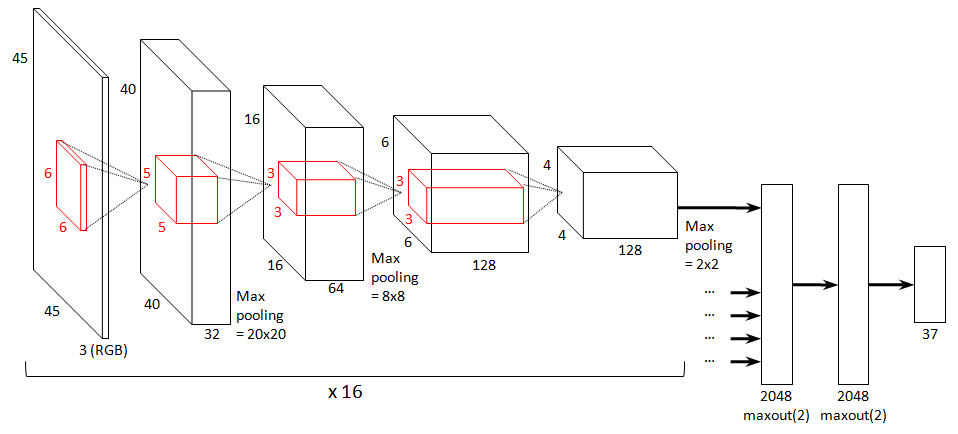
\includegraphics[width=1\textwidth]{images/deep_conv.png}
\end{figure}

\end{frame}


\begin{frame}{Very deep convolutional network}

\begin{figure}[h!]
  \centering
  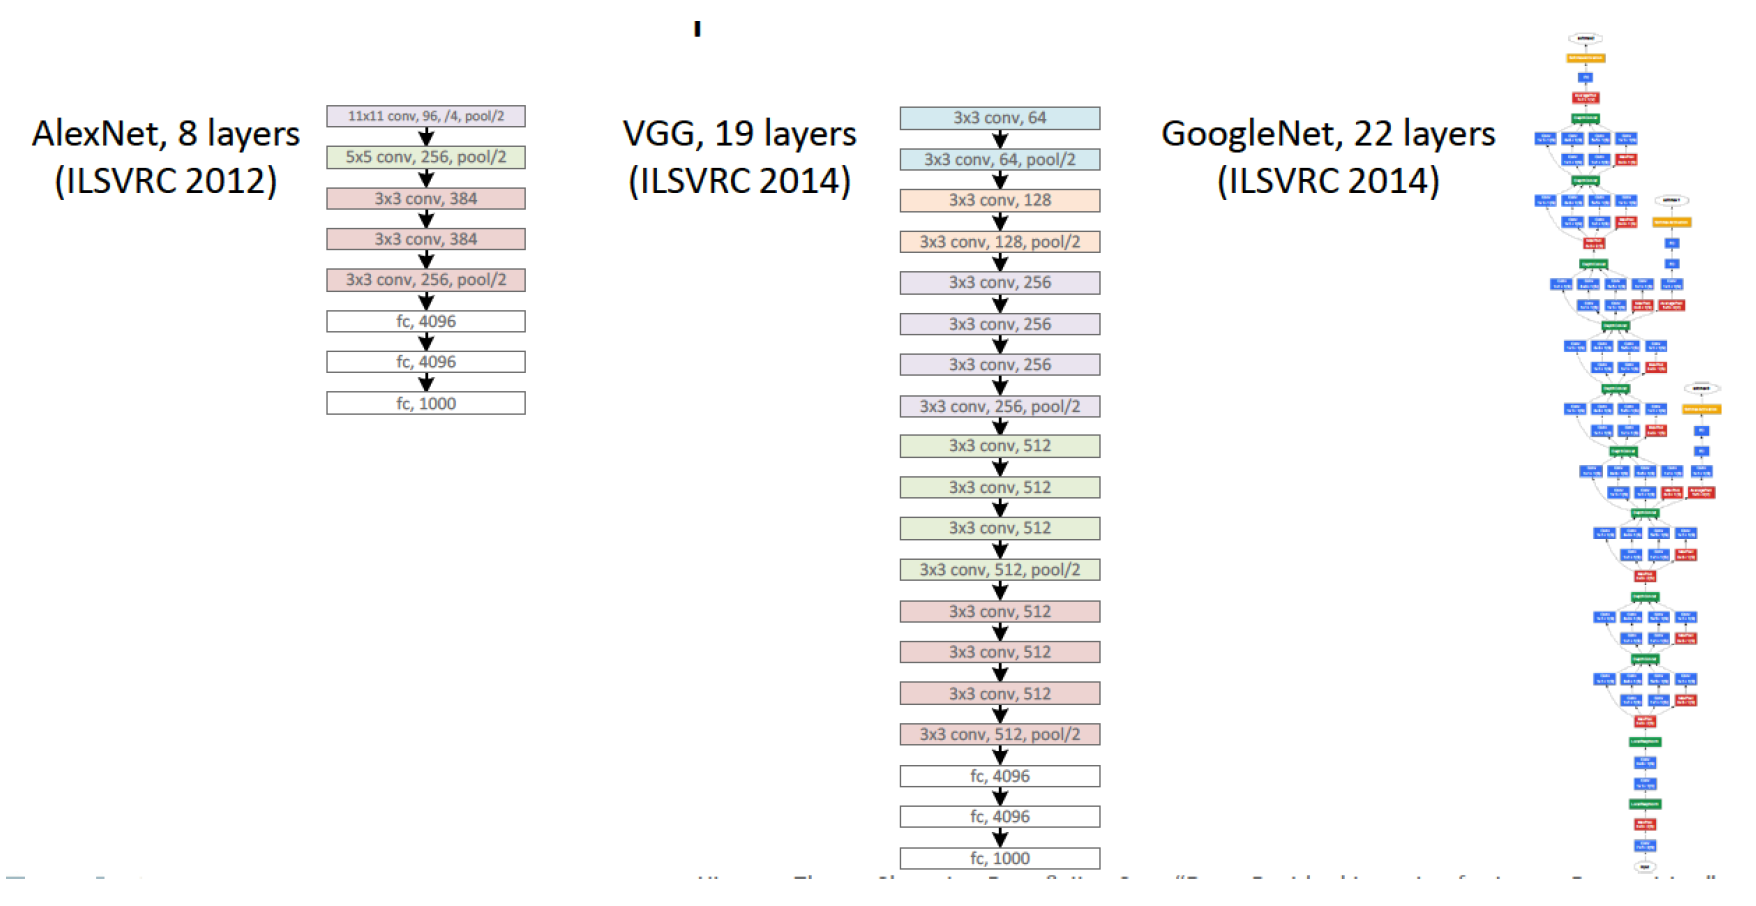
\includegraphics[width=1\textwidth]{images/comp1.png}
\end{figure}

\end{frame}


\begin{frame}{Very very deep convolutional network}

\begin{figure}[h!]
  \centering
  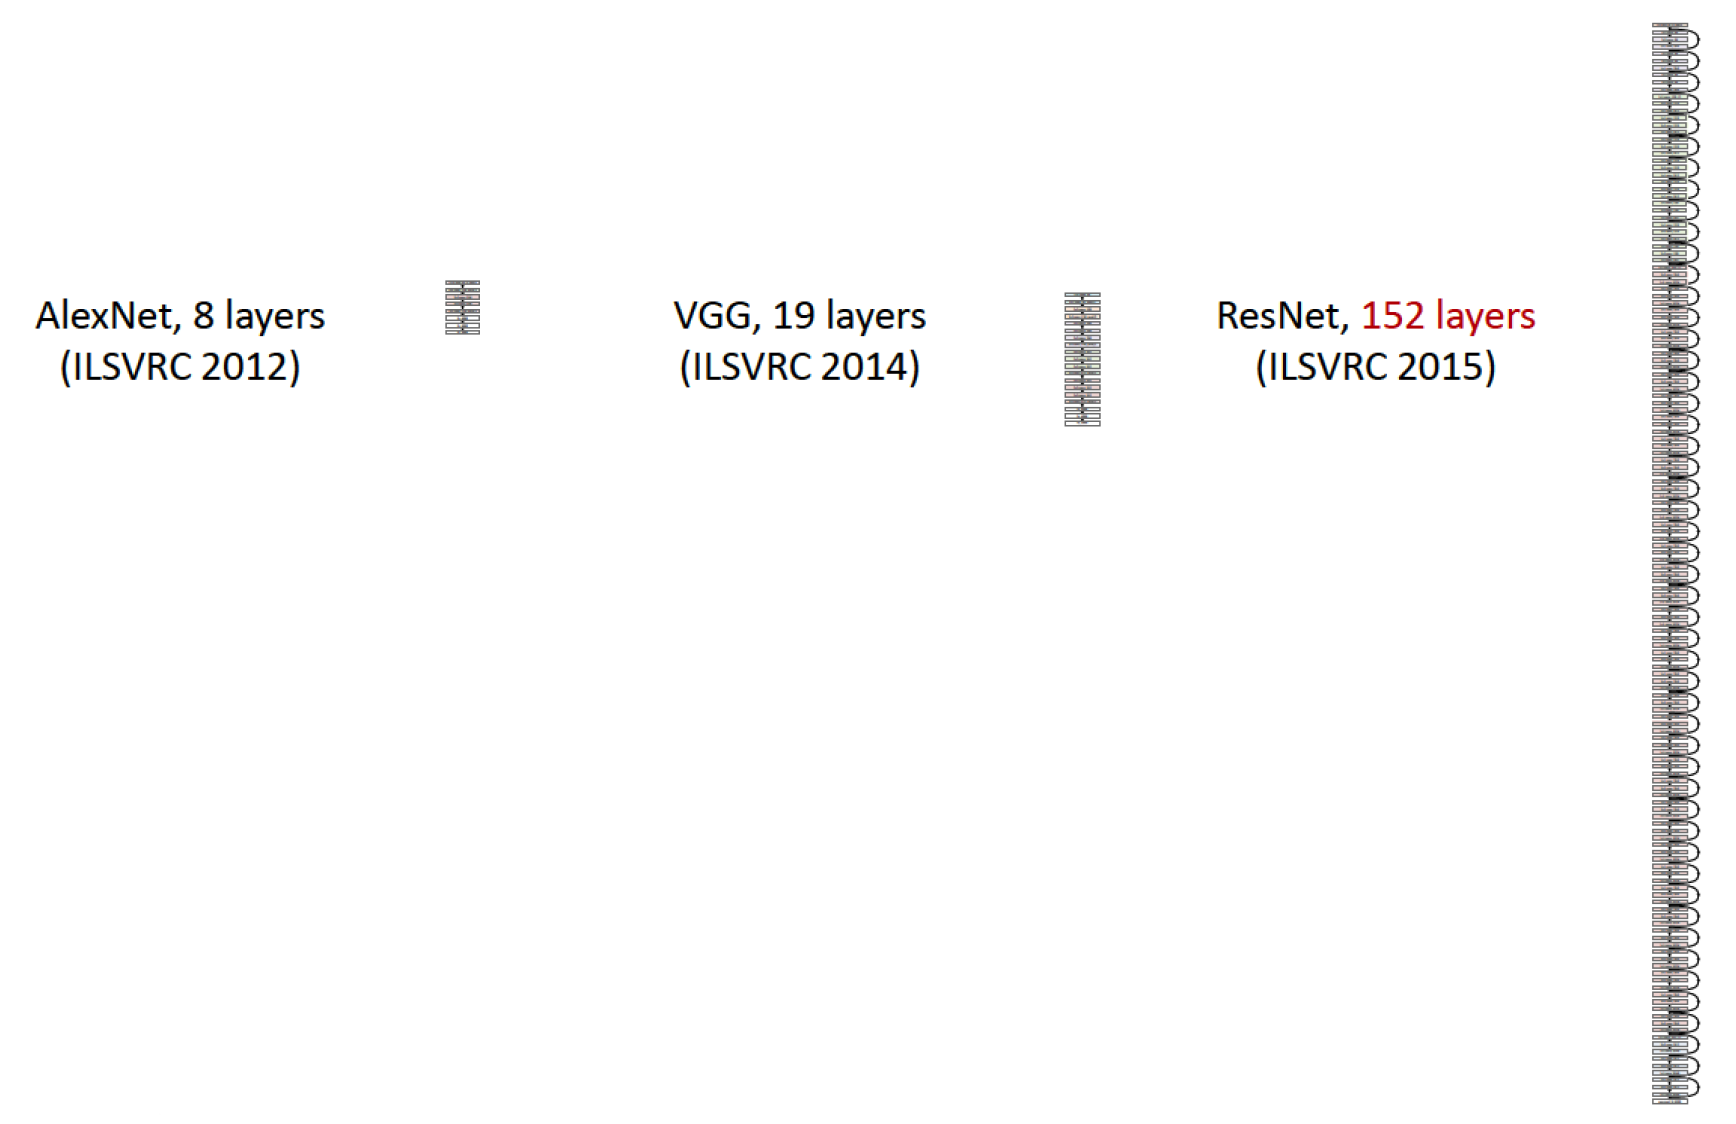
\includegraphics[width=1\textwidth]{images/comp2.png}
\end{figure}

\end{frame}


\begin{frame}{...}

\begin{figure}[h!]
  \centering
  
\includegraphics[width=1\textwidth]{images/moar.png}
\end{figure}

\end{frame}


\begin{frame}{State-of-the-art}

\begin{figure}[h!]
  \centering
  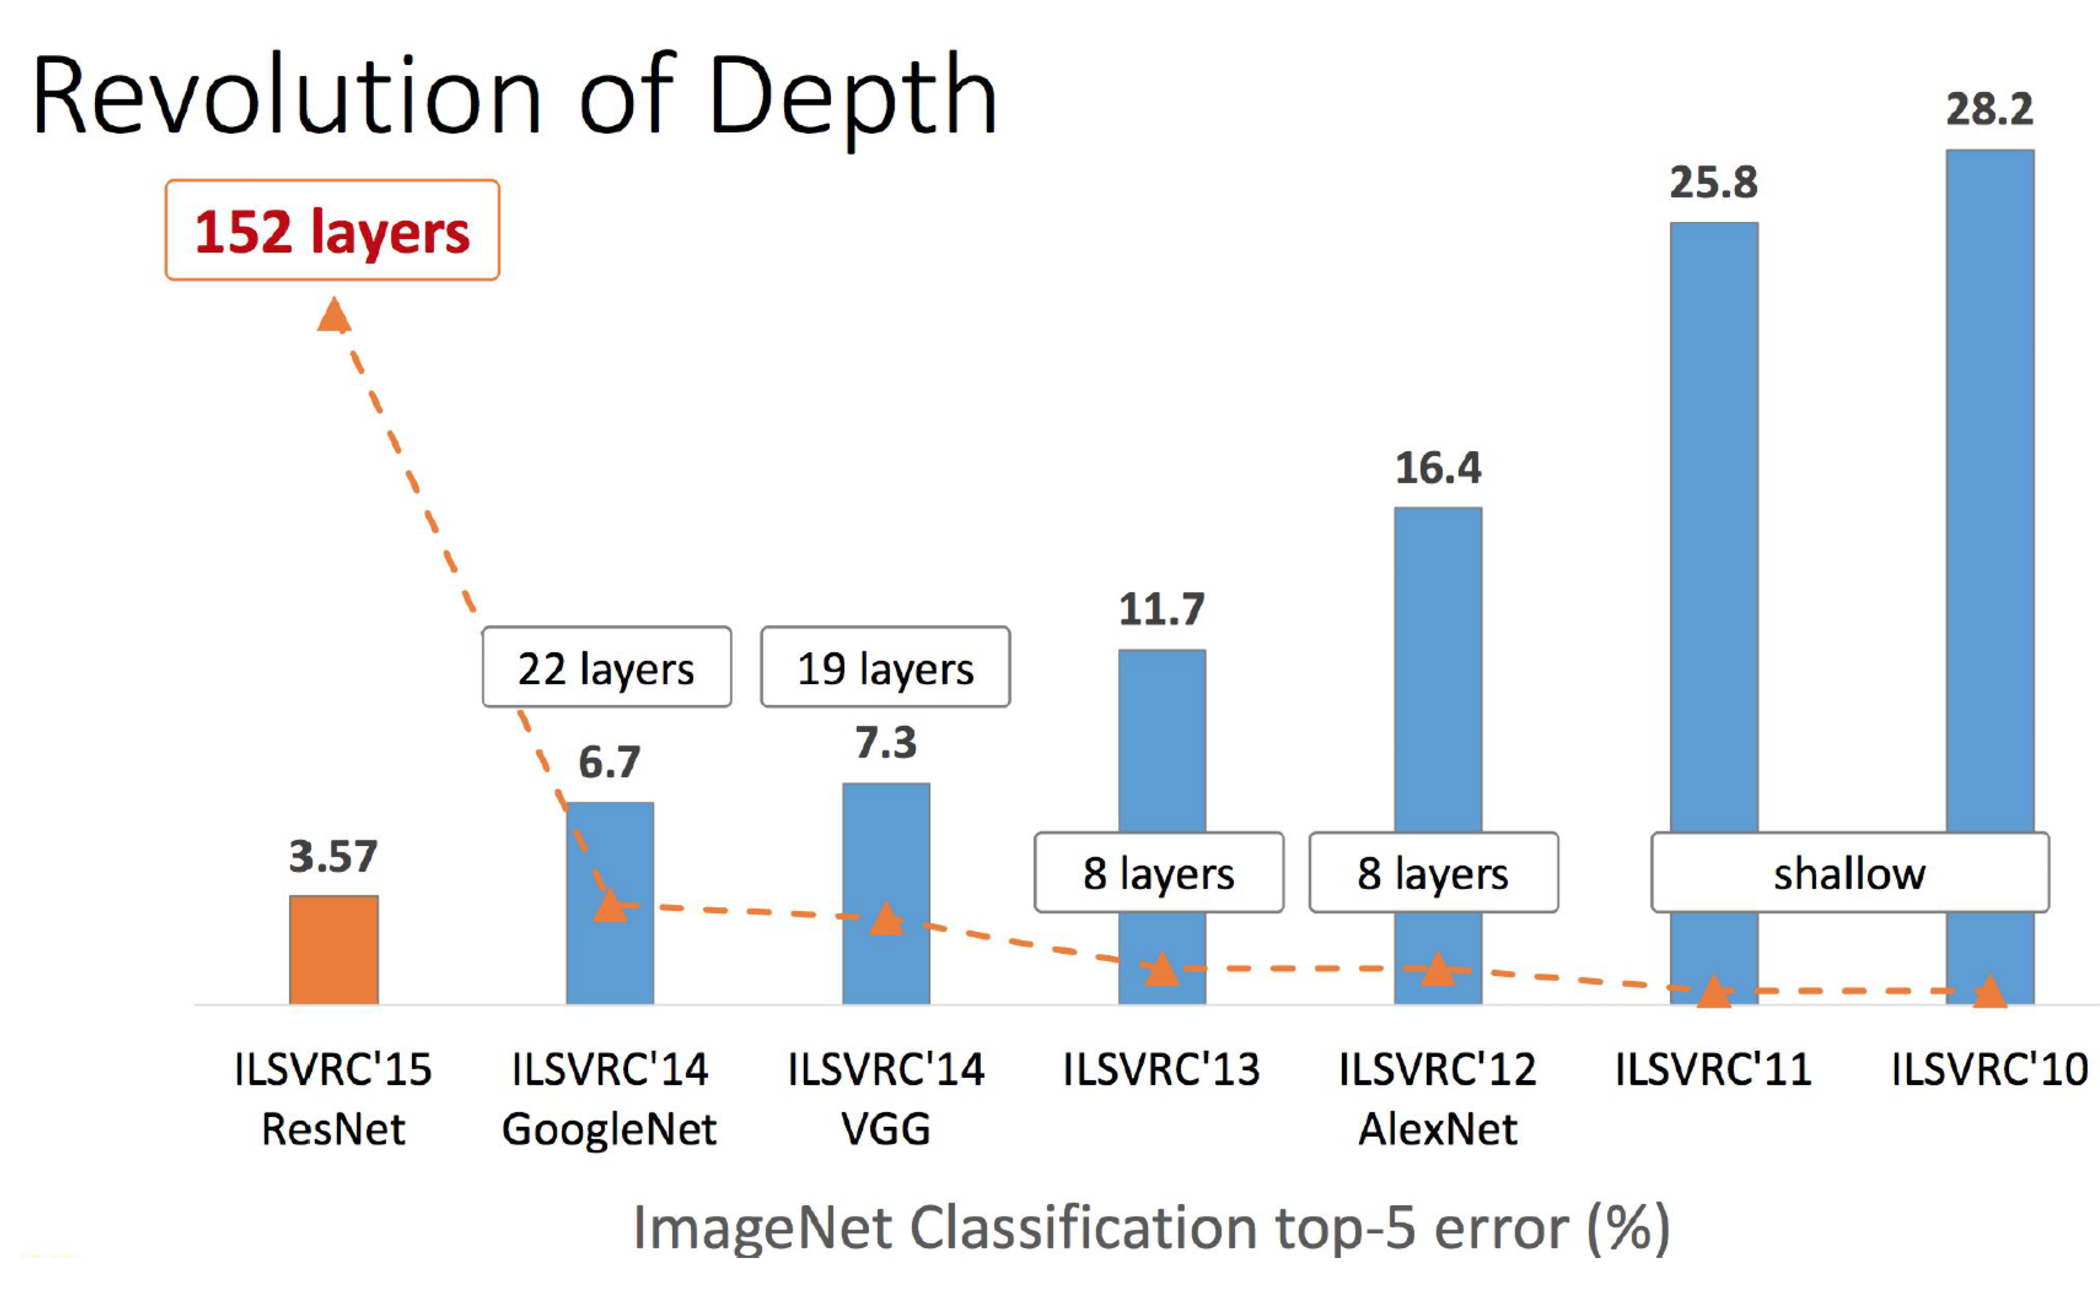
\includegraphics[width=1\textwidth]{images/rev_depth.png}
\end{figure}

\end{frame}


\begin{frame}{Deconvolution}

say about blackbox
introduce deconvolution network
may be derivative wrt image

\end{frame}


\begin{frame}{How network see the world, \#1}

\begin{figure}[h!]
  \centering
  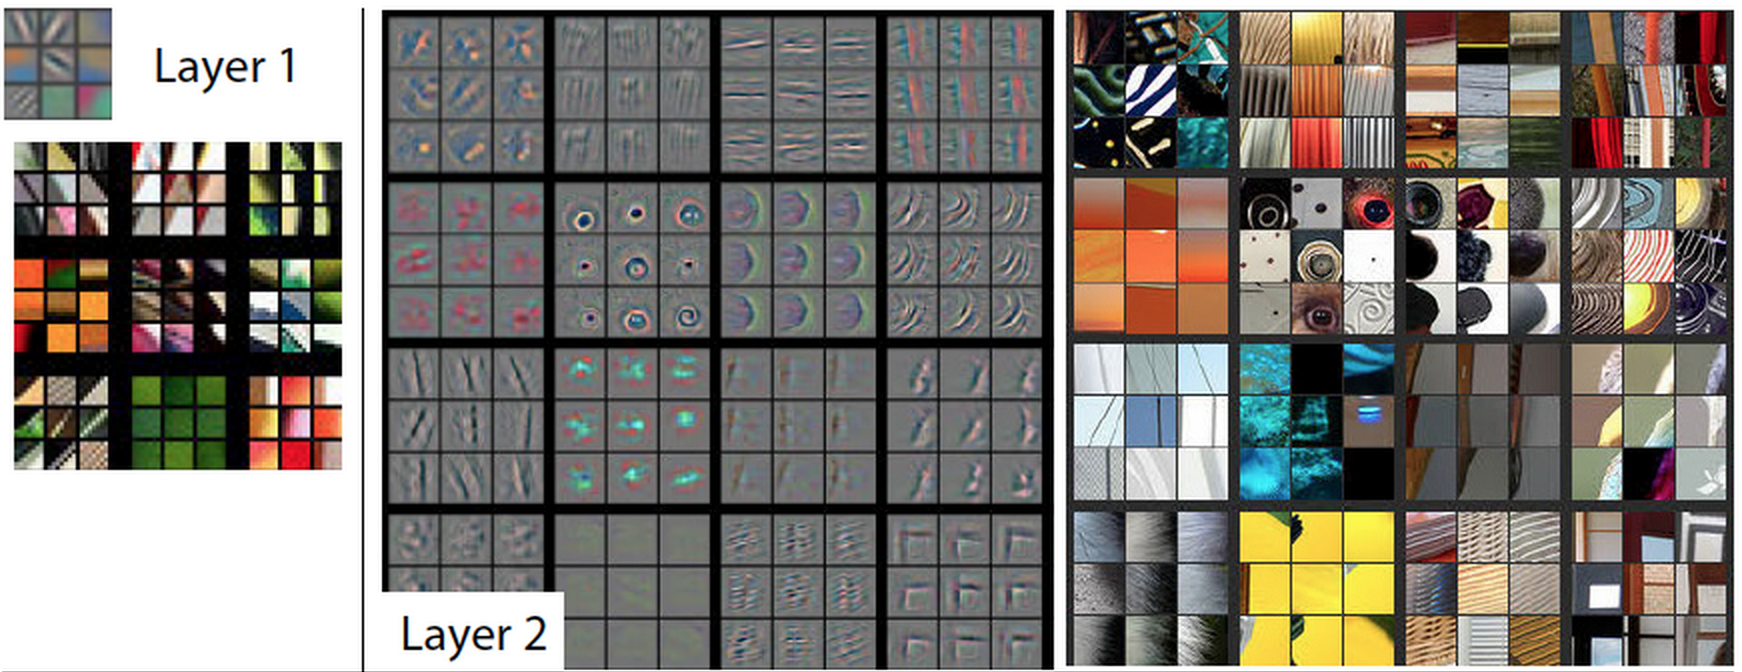
\includegraphics[width=1\textwidth]{images/features1.png}
  \caption{Visualizing and Understanding Convolutional Network \footnote{Matthew D. Zeiler and Rob Fergus}}
\end{figure}

\end{frame}


\begin{frame}{How network see the world, \#2}

\begin{figure}[h!]
  \centering
  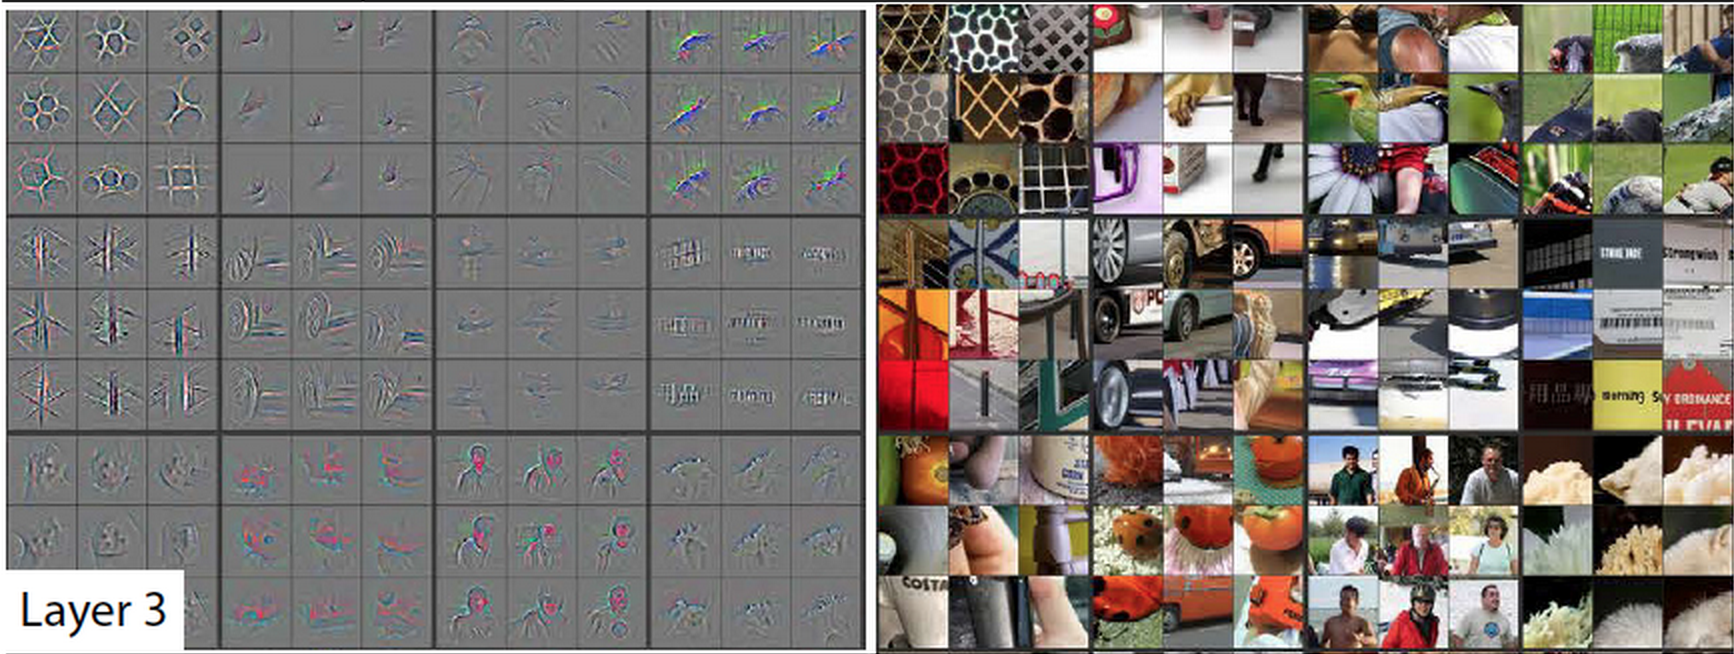
\includegraphics[width=1\textwidth]{images/features2.png}
\end{figure}

\end{frame}


\begin{frame}{How network see the world, \#3}

\begin{figure}[h!]
  \centering
  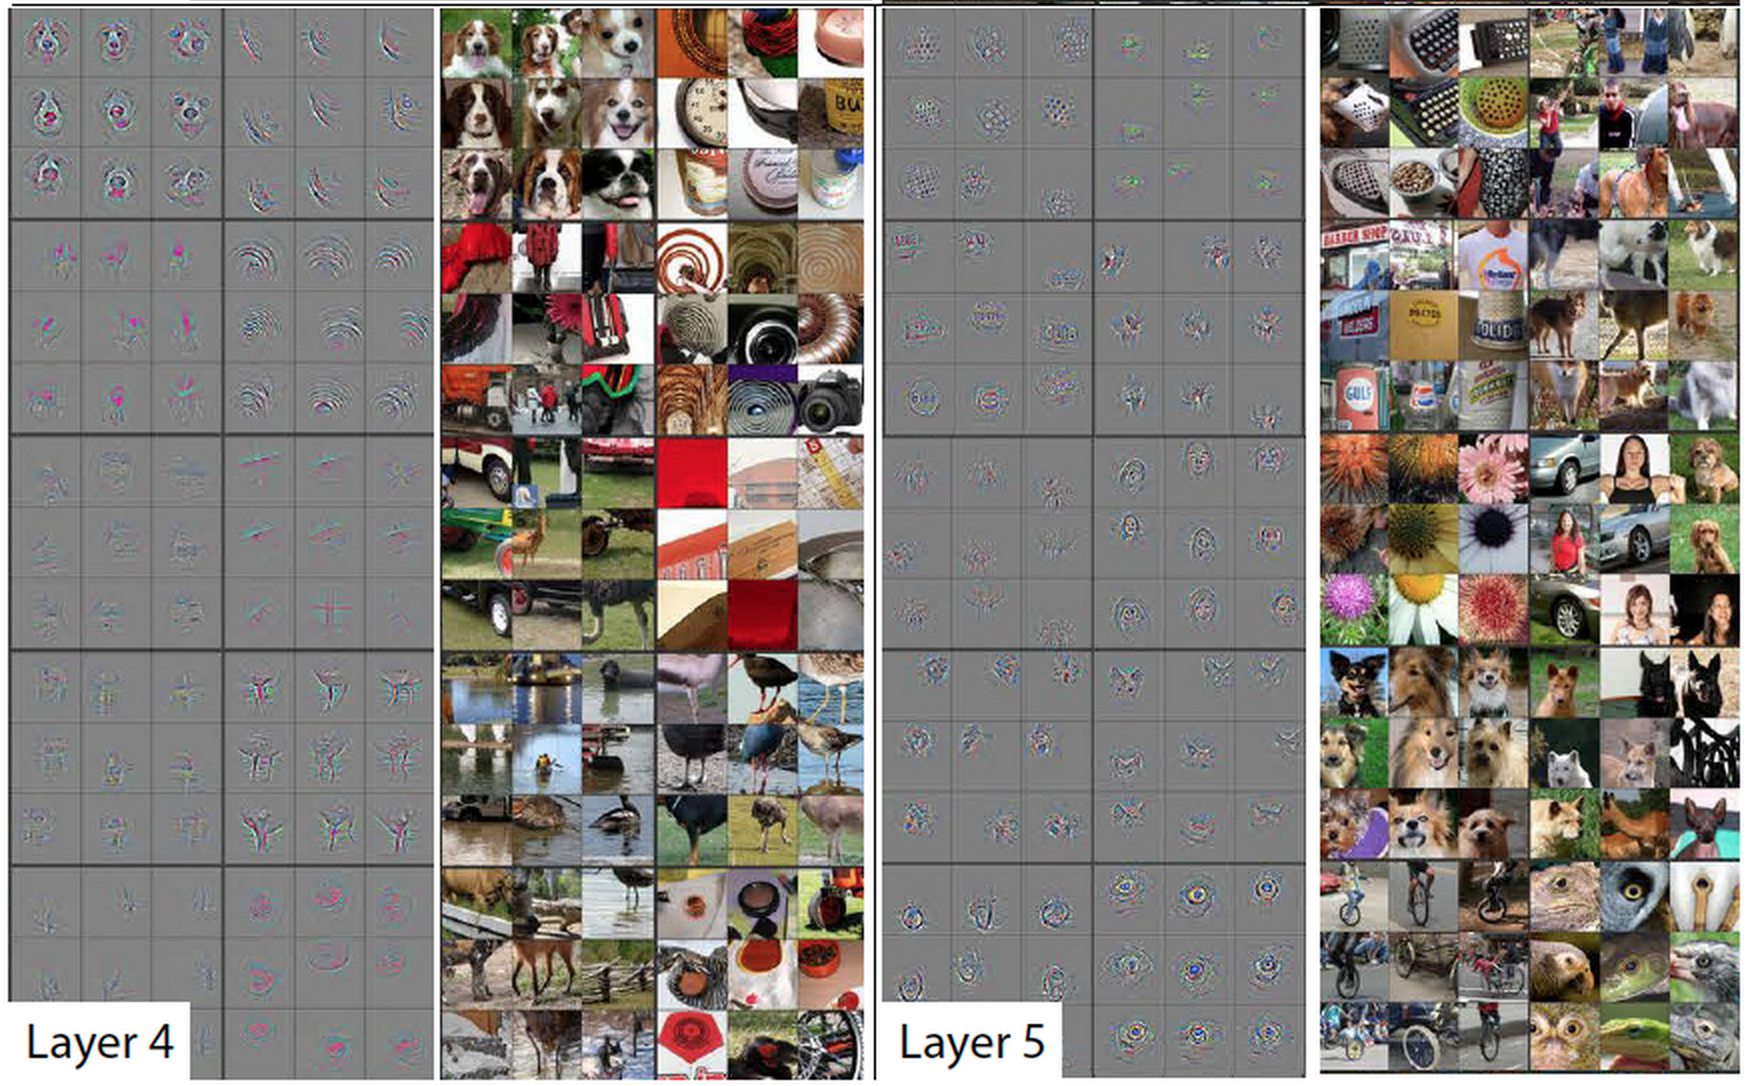
\includegraphics[width=1\textwidth]{images/features3.png}
\end{figure}

\end{frame}


\begin{frame}{Eye filter, \#1}

\begin{figure}[h!]
  \centering
  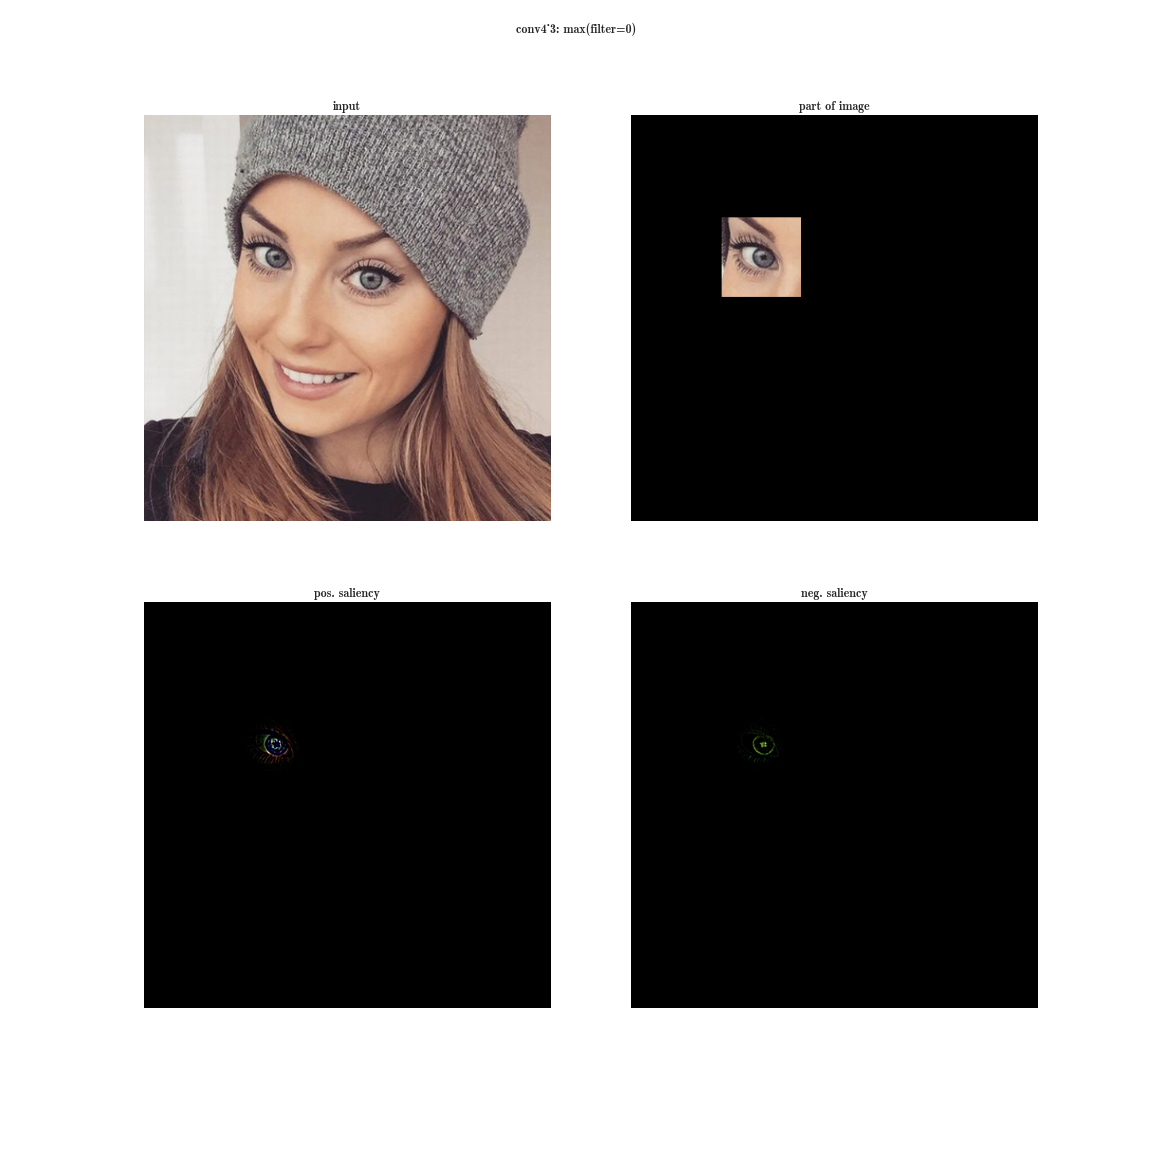
\includegraphics[width=0.9\textwidth]{images/eye1.png}
\end{figure}

\end{frame}


\begin{frame}{Eye filter, \#2}

\begin{figure}[h!]
  \centering
  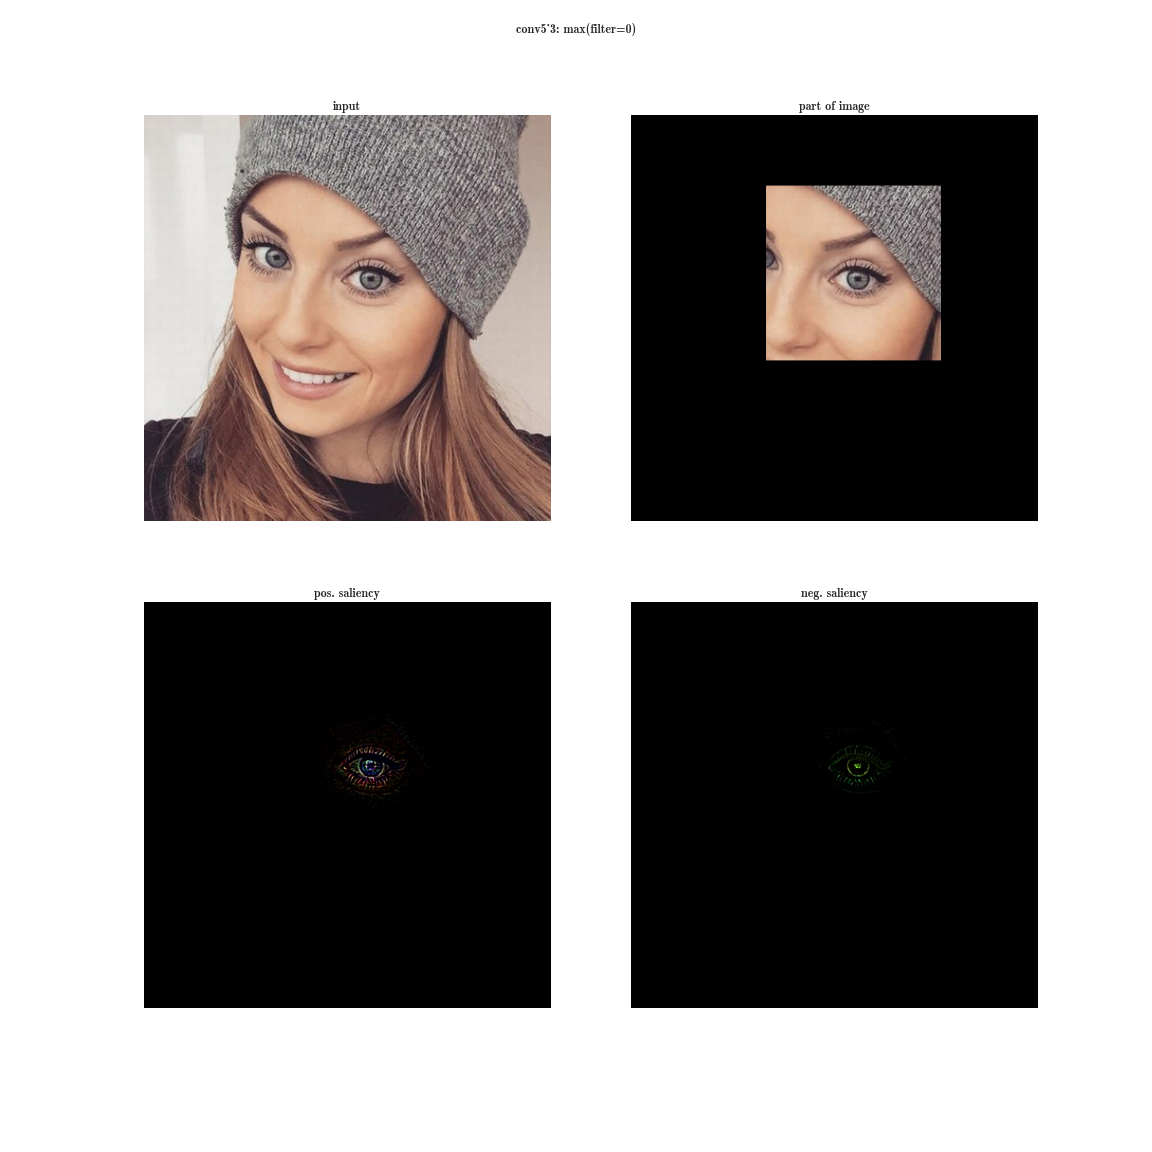
\includegraphics[width=0.9\textwidth]{images/eye2.png}
\end{figure}

\end{frame}


\begin{frame}{Deep learning = Representation learning}

\begin{figure}[h!]
  \centering
  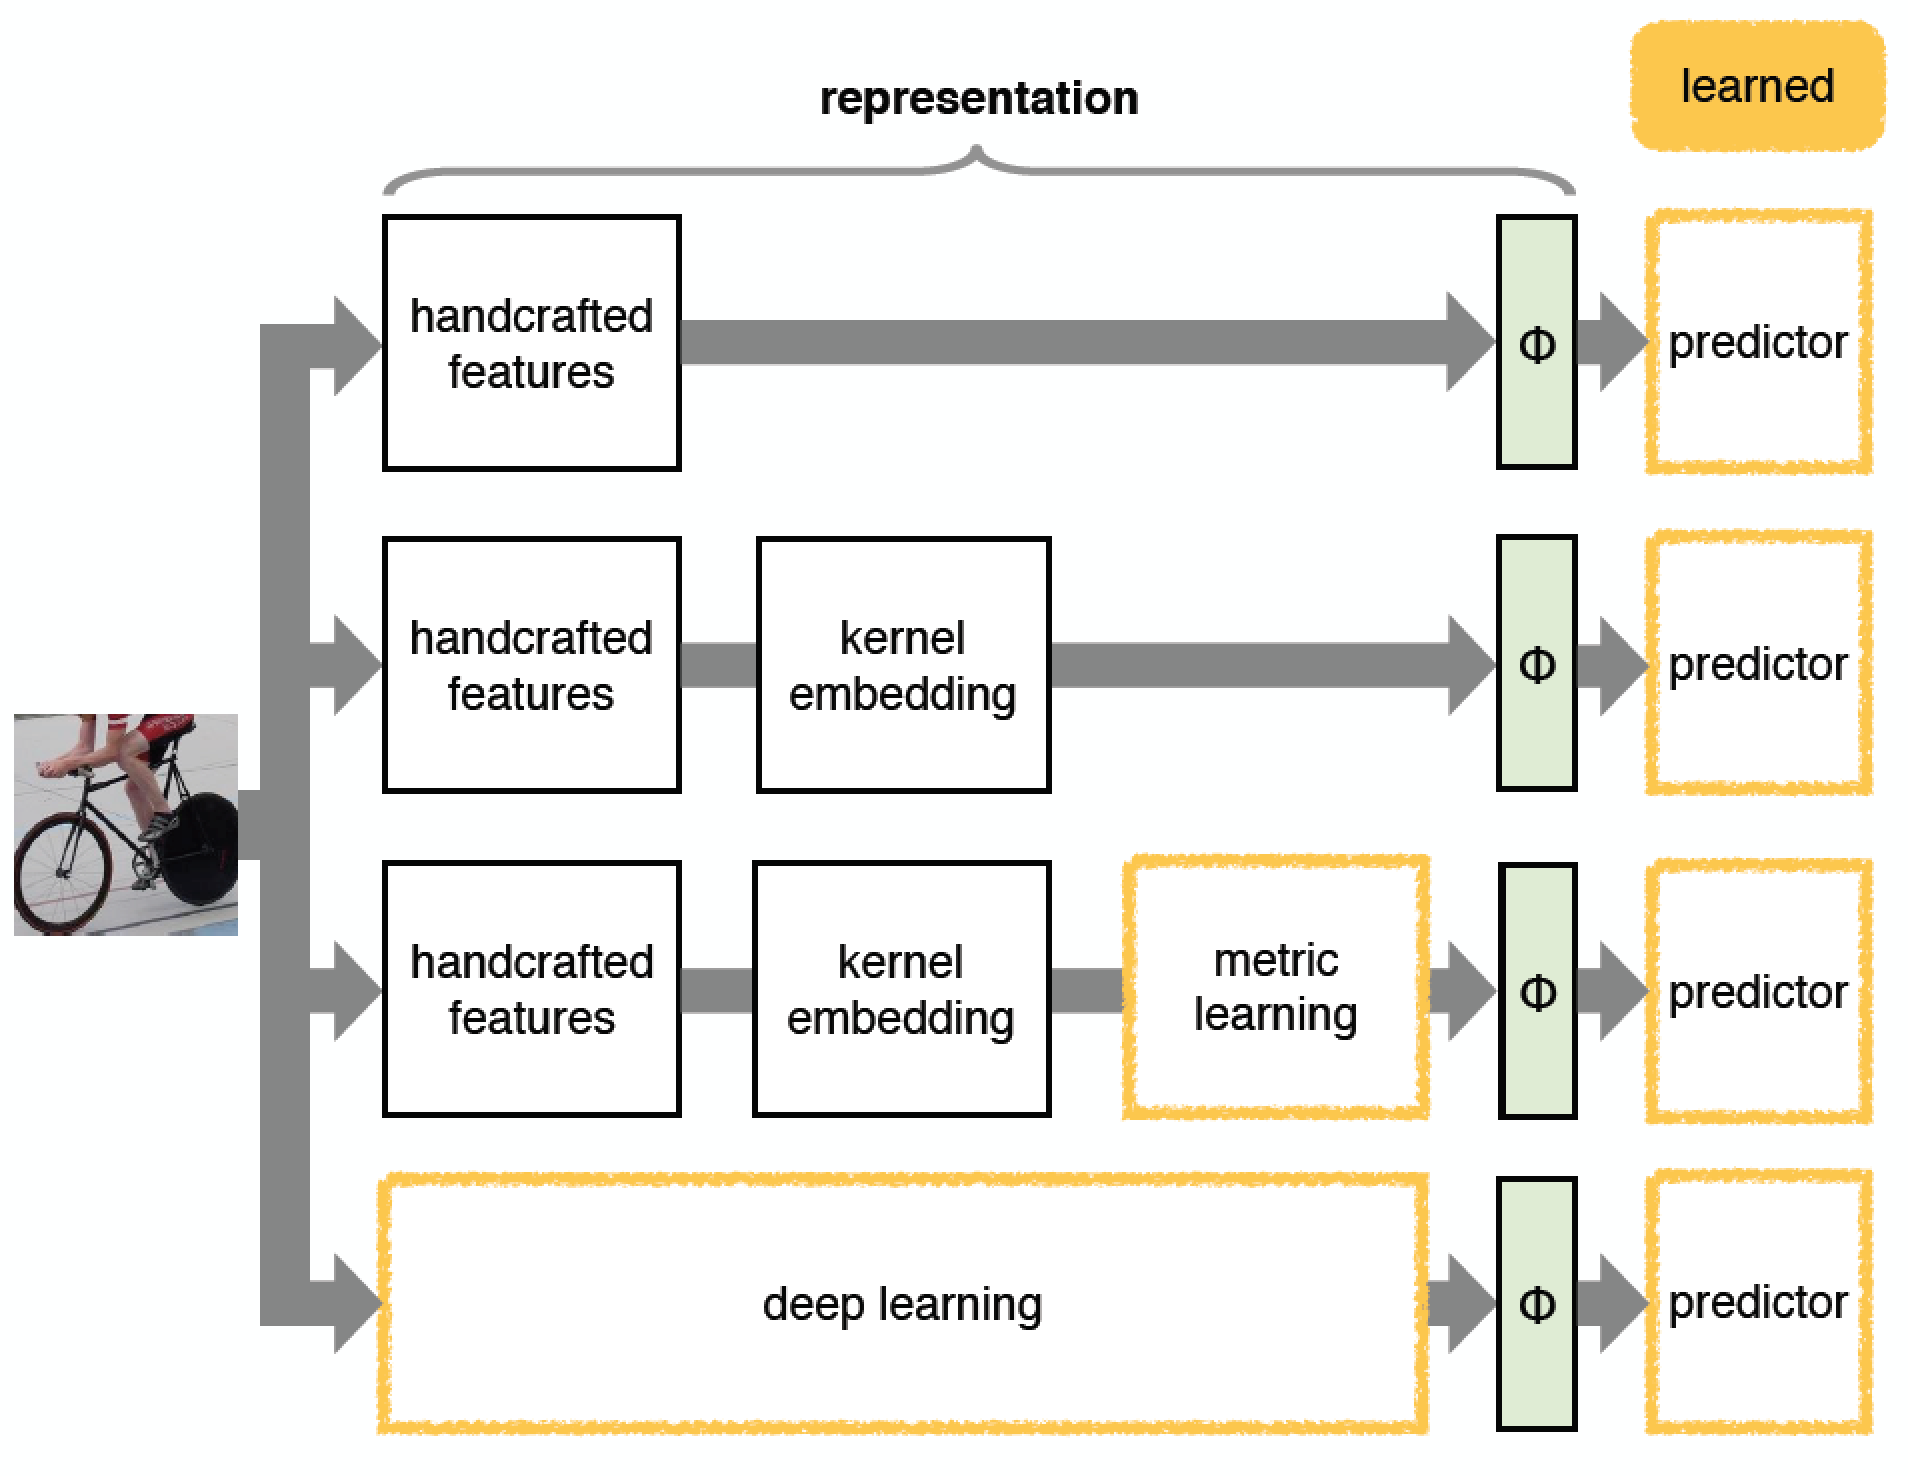
\includegraphics[width=1\textwidth]{images/ife.png}
\end{figure}

\end{frame}



\begin{frame}{Semantic hashing}

\begin{figure}[h!]
  \centering
  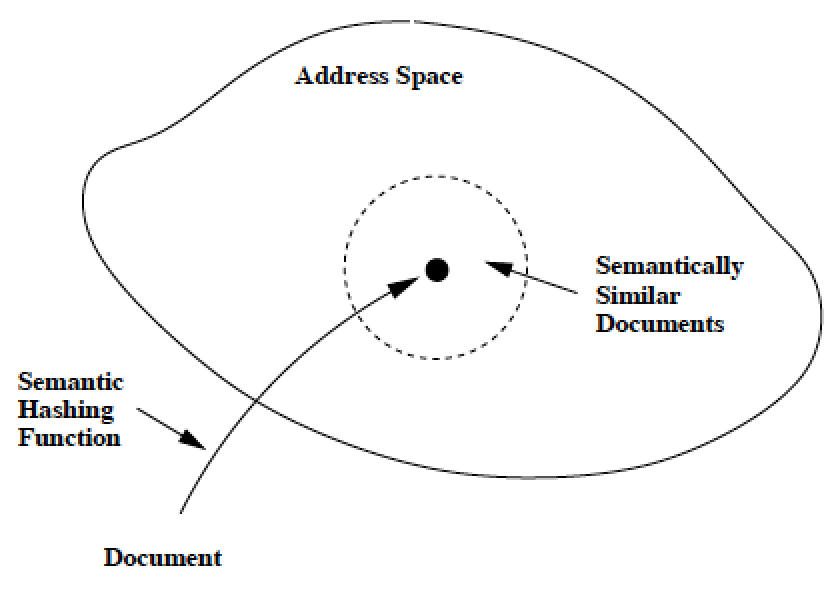
\includegraphics[width=0.9\textwidth]{images/sh_schema.png}
  \caption{Semantic representation\footnote{Semantic Hashing (Salakhutdinov, Hinton)}}
\end{figure}

\end{frame}


\begin{frame}{Deep sparse autoencoder}

\begin{figure}[h!]
  \centering
  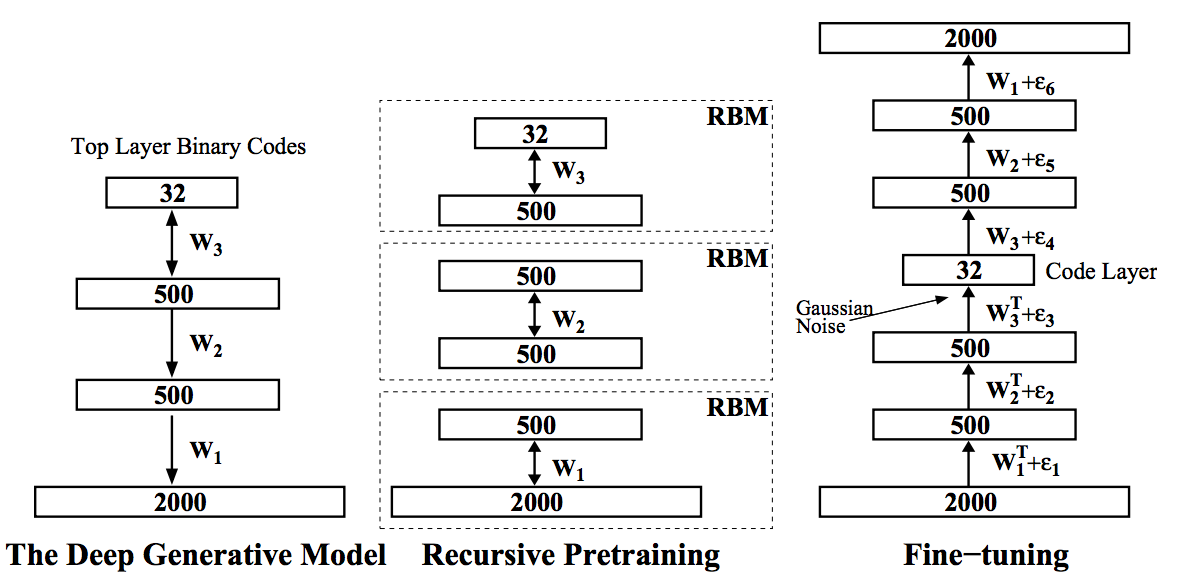
\includegraphics[width=1\textwidth]{images/dae.png}
  \caption{Training of deep autoencoder\footnote{Semantic Hashing (Salakhutdinov, Hinton)}}
\end{figure}

\end{frame}


\begin{frame}{Compression}

\begin{figure}[h!]
  \centering
  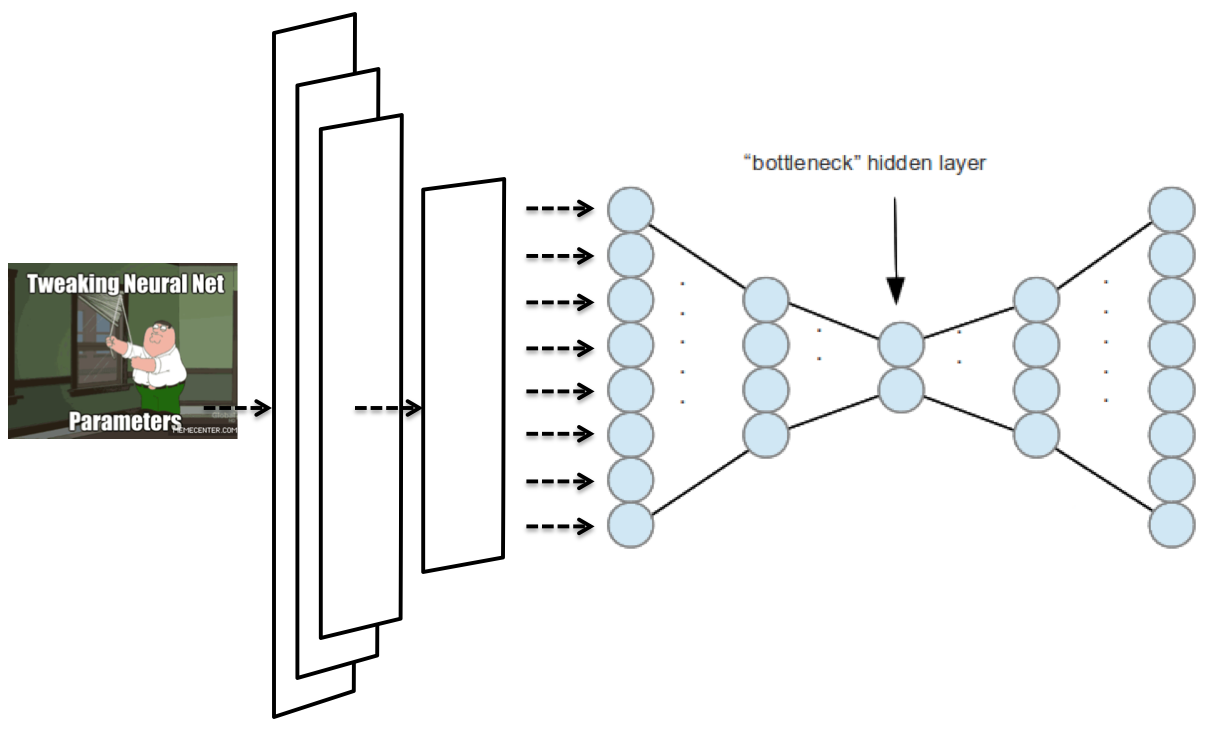
\includegraphics[width=1\textwidth]{images/vgg_transfer_sh.png}
\end{figure}

\end{frame}


\begin{frame}{Visualization, \#1}

\begin{figure}[h!]
  \centering
  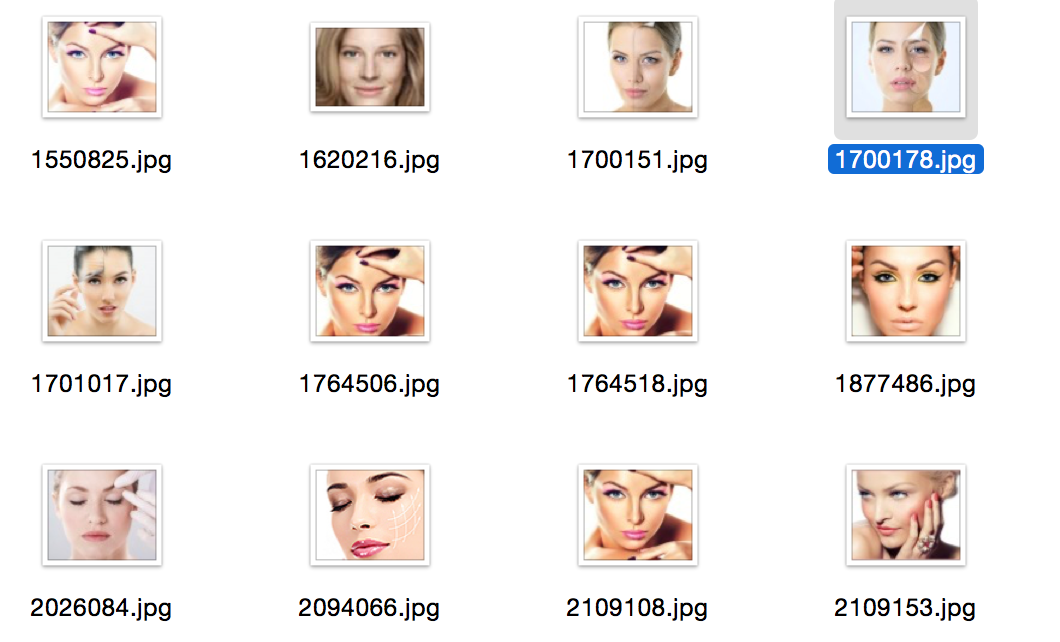
\includegraphics[width=1\textwidth]{images/search1.png}
\end{figure}

\end{frame}


\begin{frame}{Visualization, \#2}

\begin{figure}[h!]
  \centering
  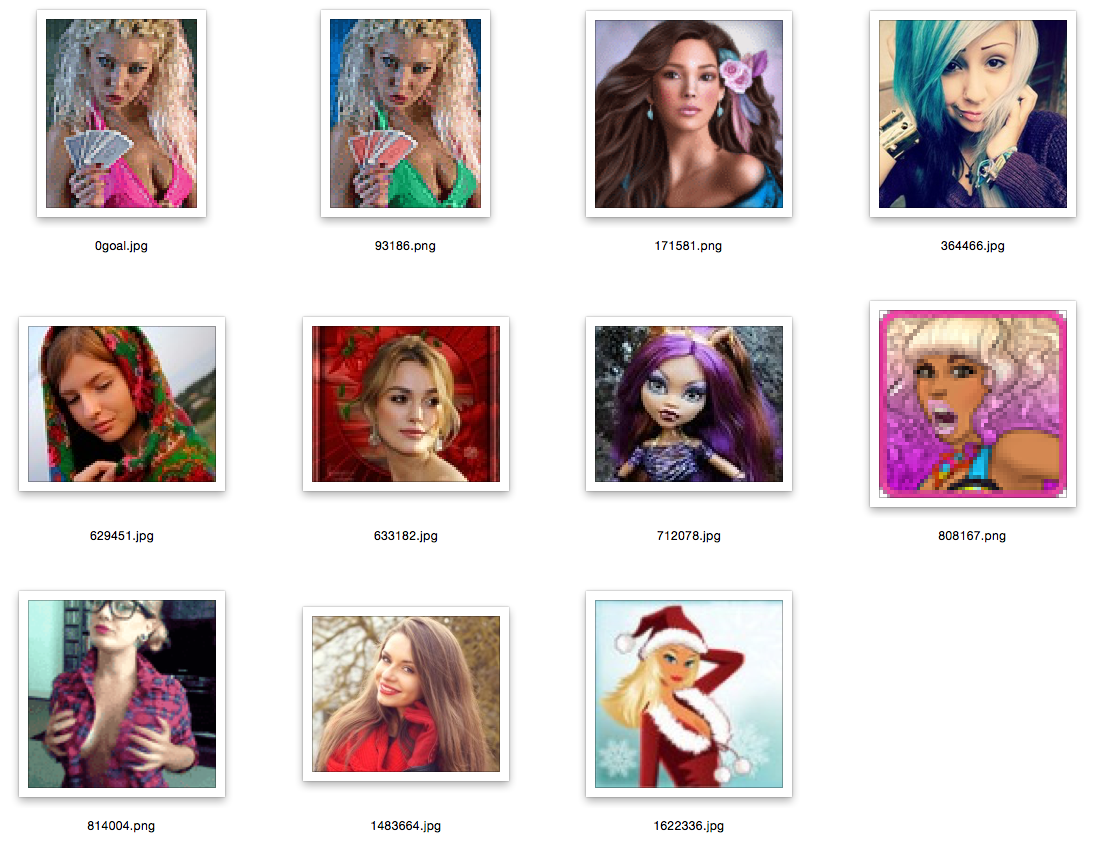
\includegraphics[width=1\textwidth]{images/search2.png}
\end{figure}

\end{frame}


\begin{frame}{Visualization, \#3}

\begin{figure}[h!]
  \centering
  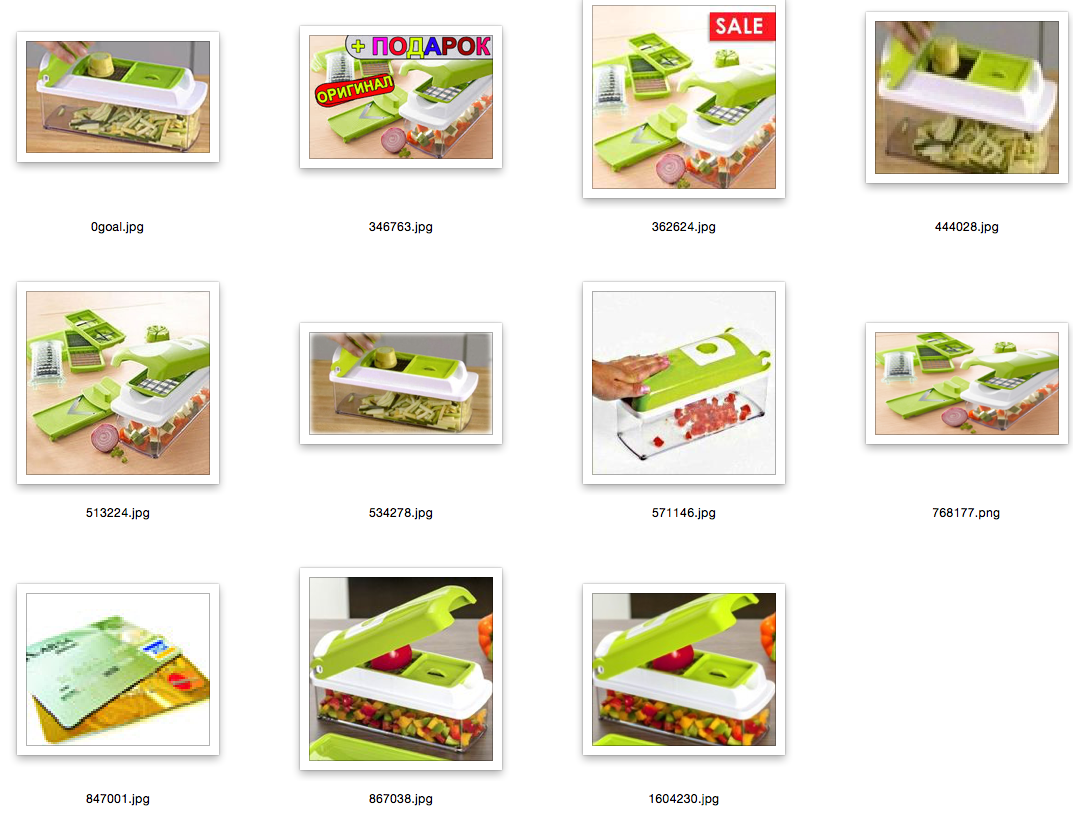
\includegraphics[width=1\textwidth]{images/search3.png}
\end{figure}

\end{frame}


\begin{frame}{Visualization, \#4}

\begin{figure}[h!]
  \centering
  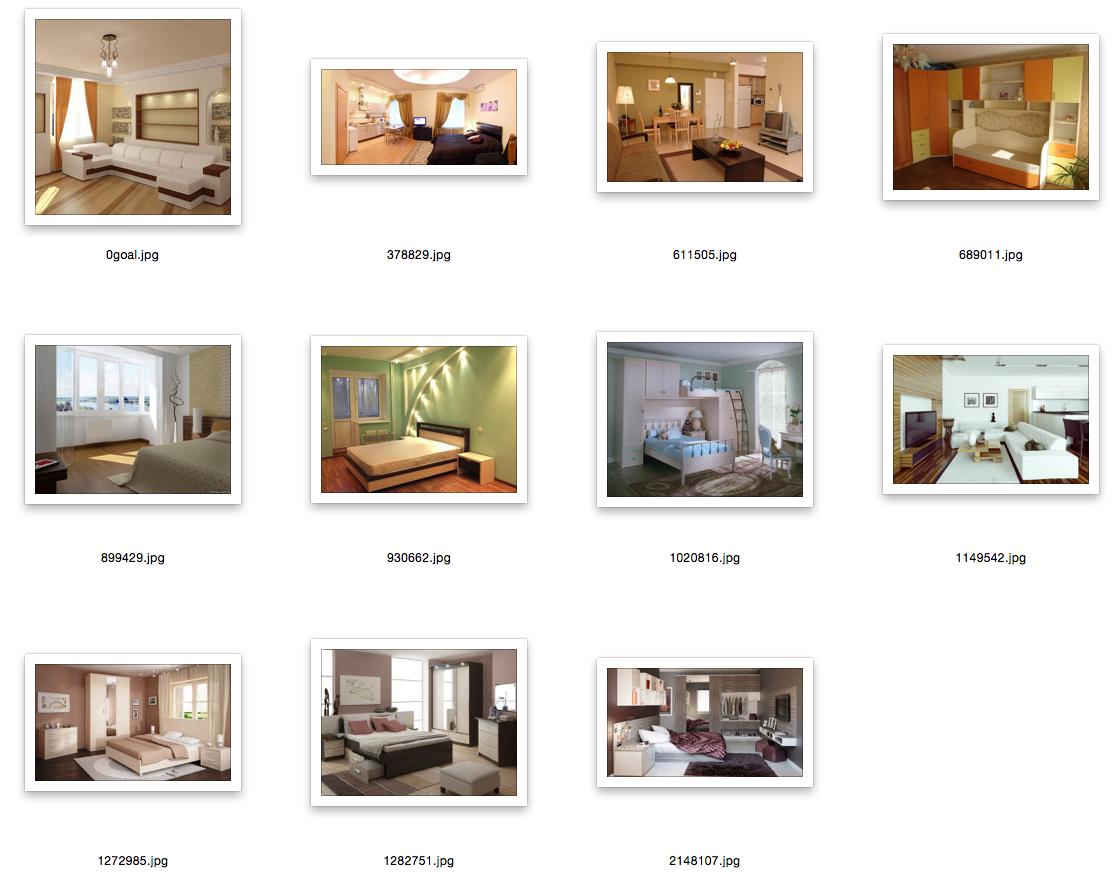
\includegraphics[width=1\textwidth]{images/search4.png}
\end{figure}

\end{frame}


\begin{frame}{Visualization, \#5}

\begin{figure}[h!]
  \centering
  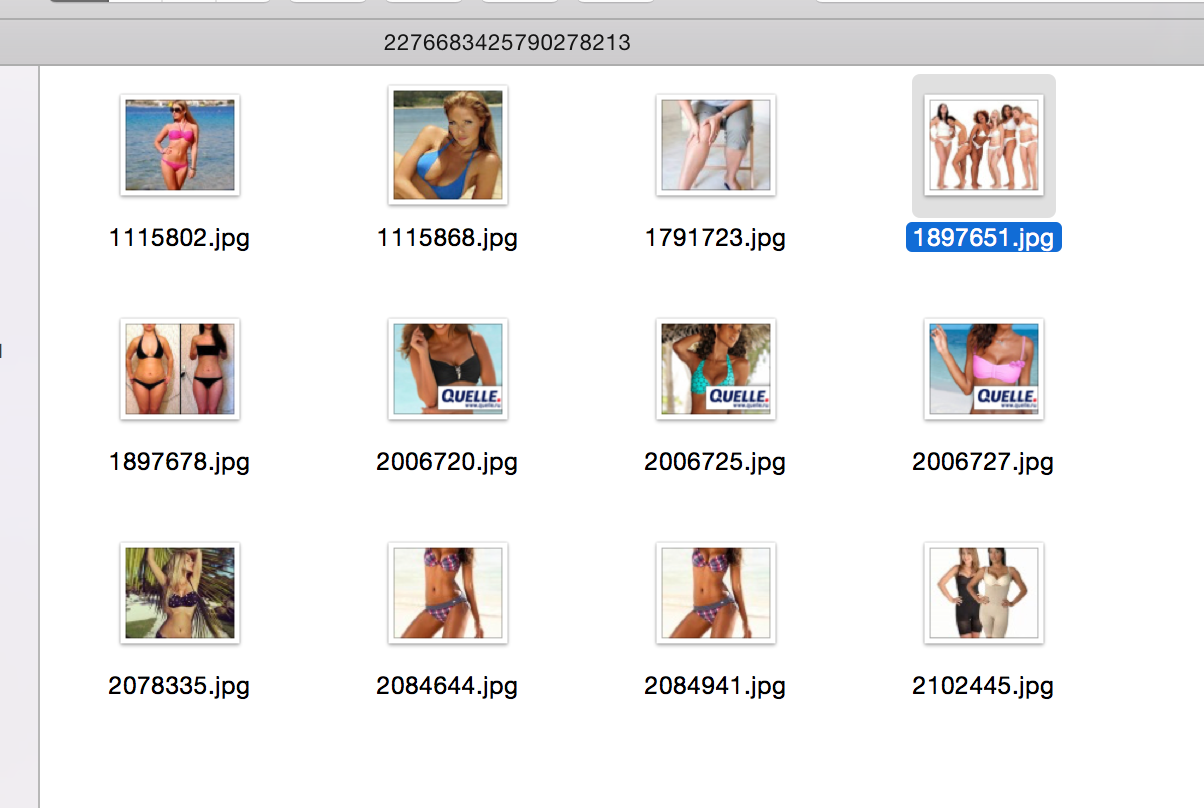
\includegraphics[width=1\textwidth]{images/search5.png}
\end{figure}

\end{frame}


\begin{frame}{Visualization, \#6}

\begin{figure}[h!]
  \centering
  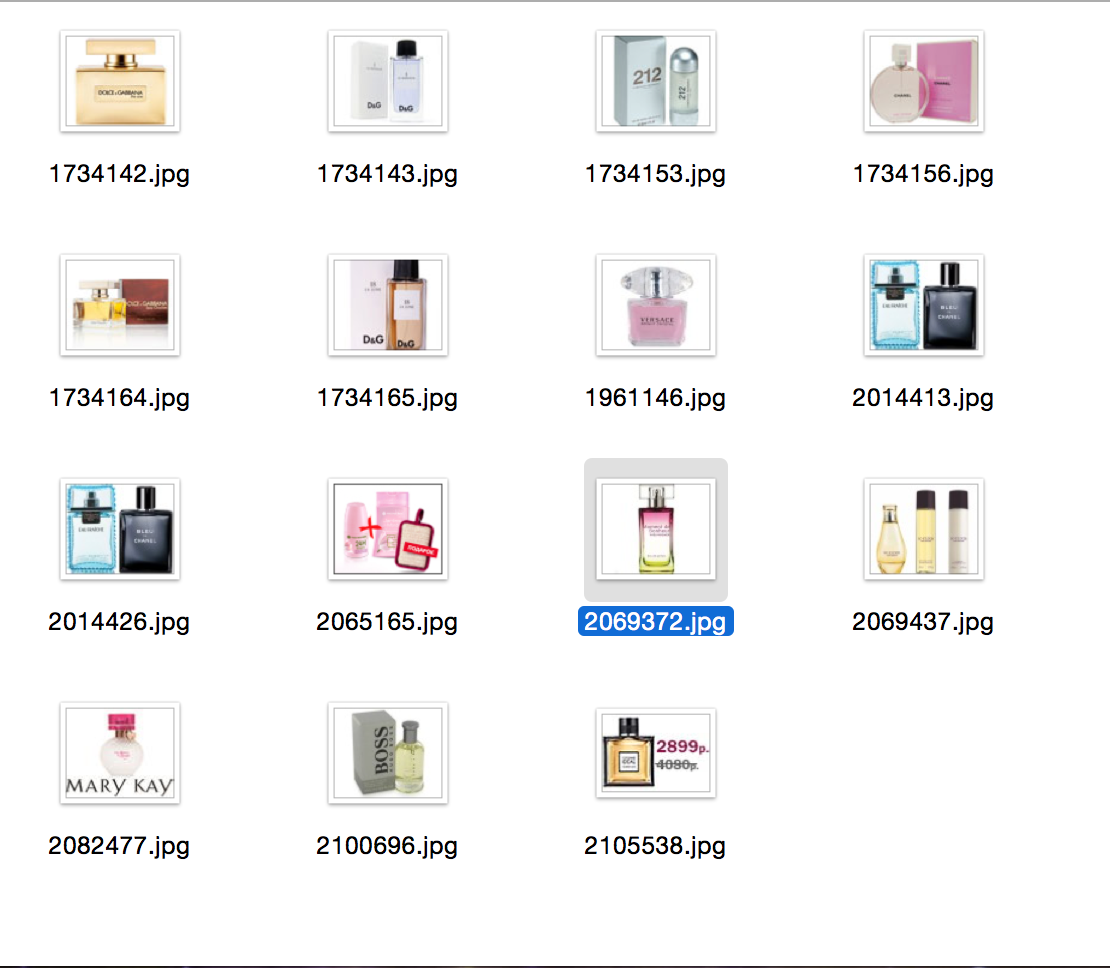
\includegraphics[width=1\textwidth]{images/search6.png}
\end{figure}

\end{frame}


\begin{frame}{Visualization, \#7}

\begin{figure}[h!]
  \centering
  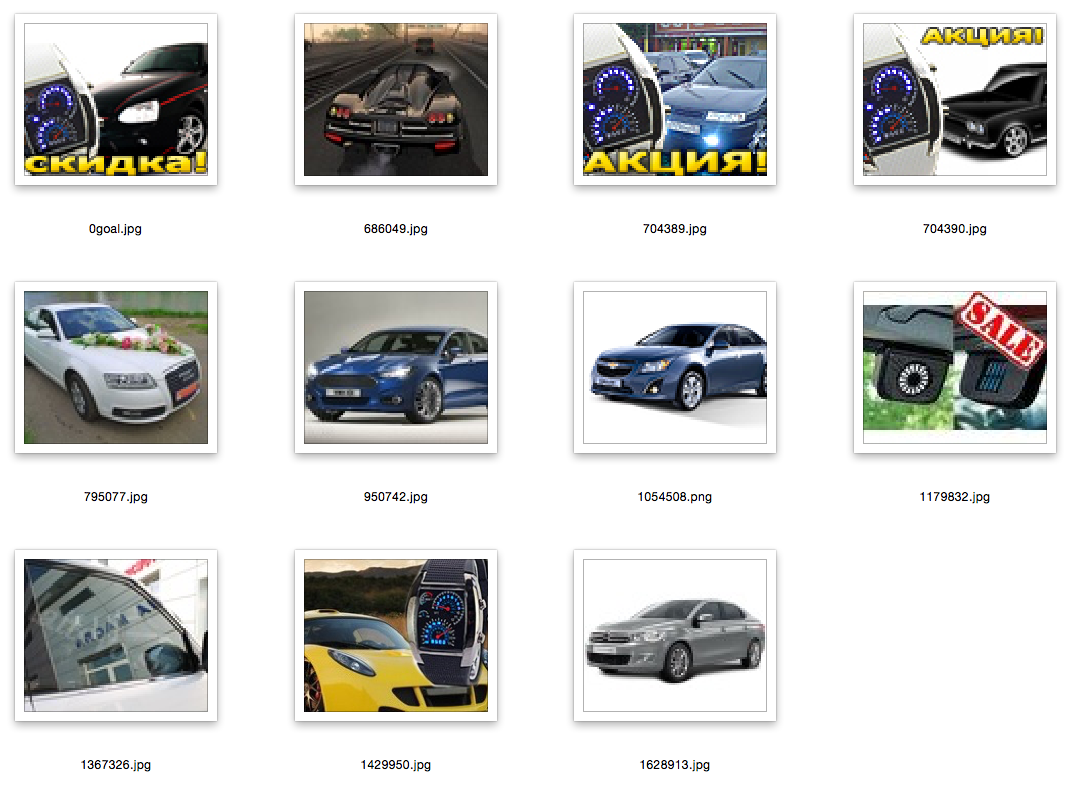
\includegraphics[width=1\textwidth]{images/search7.png}
\end{figure}

\end{frame}




\begin{comment}
\begin{itemize}
  \item Your introduction goes here!
  \item Use \texttt{itemize} to organize your main points.
\end{itemize}
\vskip 1cm
\begin{block}{Examples}
Some examples of commonly used commands and features are included, to help you get started.
\end{block}
\end{comment}


\end{document}